\subsection{Interrelación Asignatura Curso Académico - Alumno Curso Académico}

   \begin{description}
      \item[Definición] En esta interrelación se deja constancia de que un
      alumno está matriculado de un determinado número de asignaturas en un
      curso académico.

      \item[Características] La interrelación presenta las siguientes
                             características:

         \begin{itemize}
            \item \textbf{Nombre:} ACA-AlCA
            \item \textbf{Tipo de la interrelación:} Fuerte.
            \item \textbf{Cardinalidad de la interrelación:} N:M
                  \begin{itemize}
                     \item Asignatura Curso Académico: dispone\_de (0,n)
                     \item Alumno Curso Académico: matriculado\_en (0,n)
                  \end{itemize}
            \item \textbf{Número de atributos:} Tres: convocatoria, nota y
                  comentario.
         \end{itemize}

      \item[Diagrama] La figura \ref{diagramaACA-AlCA} muestra el diagrama de la
                      interrelación.

       \item \begin{figure}[!ht]
            \begin{center}
            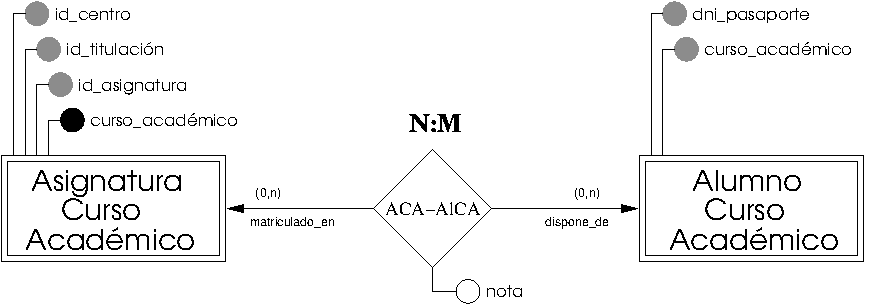
\includegraphics[]{07.Modelo_Entidad-Interrelacion/7.3.Analisis_Interrelaciones/diagramas/ACA-AlCA.pdf}
            \caption{Diagrama de la interrelación ACA-AlCA.}
            \label{diagramaACA-AlCA}
            \end{center}
         \end{figure}

      \item[Descripción de los atributos] La interrelación presenta los
      siguientes atributos:

       \begin{itemize}
        \item \textbf{convocatoria}
          \begin{itemize}
            \item \textbf{Definición:} Establece la convocatoria en la que el
            alumno se presenta a la asignatura.
            \item \textbf{Dominio:} Conjunto de caracteres alfanuméricos.
            \item \textbf{Carácter:} Obligatorio.
            \item \textbf{Ejemplo práctico:} febrero.
            \item \textbf{Información adicional:} Es clave primaria de la
            interrelación. El dato \textbf{¿¿QUIÉN LO INTRODUCE??}.
         \end{itemize}
         \item \textbf{nota}
          \begin{itemize}
            \item \textbf{Definición:} Establece la calificación obtenida por un
            alumno en una asignatura durante un curso académico.
            \item \textbf{Dominio:} Conjunto de reales positivos.
            \item \textbf{Carácter:} Opcional.
            \item \textbf{Ejemplo práctico:} 8,4.
            \item \textbf{Información adicional:} El dato \textbf{¿¿QUIÉN LO INTRODUCE??}.
         \end{itemize}
          \item \textbf{comentario}
          \begin{itemize}
            \item \textbf{Definición:} Información extra que sea interesante
            conocer.
            \item \textbf{Dominio:} Conjunto de caracteres alfanuméricos.
            \item \textbf{Carácter:} Opcional.
            \item \textbf{Ejemplo práctico:} Prácticas superadas.
            \item \textbf{Información adicional:} El dato \textbf{¿¿QUIÉN LO INTRODUCE??}.
         \end{itemize}
       \end{itemize}

      \item[Ejemplo práctico del tipo de interrelación]

      \item \begin{center}
            \begin{tabular}{ | r r | }
            \hline
            \multicolumn{2}{ | c | }{\textbf{Tipo de interrelación ACA-AlCA}} \\
            \hline
            \textbf{Asignatura Curso Académico} & \\
            id\_centro & 15 \\
            id\_titulación & 3 \\
            id\_asignatura & 17 \\
            curso\_académico & 2008\\
            \hline
            \textbf{Alumno Curso Académico} & \\
            dni\_pasaporte & 01234567A \\
            curso\_académico & 2008 \\
            \hline
            \textbf{Atributos} & \\
            convocatoria & febrero \\
            nota & 8,4 \\
            comentario & Prácticas superadas \\
            \hline
            \end{tabular}
         \end{center}
   \end{description}
